\documentclass[a4paper,oneside,12pt]{extreport}

\usepackage{mmap}
\usepackage[T2A]{fontenc}
\usepackage[utf8]{inputenc}
\usepackage[english,russian]{babel}

% Текст отчёта следует печатать, соблюдая следующие размеры полей:
% левое — 30 мм, правое — 15 мм, верхнее и нижнее — 20 мм.
\usepackage[left=20mm, right=15mm, top=15mm, bottom=15mm]{geometry}

% \setlength{\parindent}{1.25cm} % Абзацный отступ

\usepackage{setspace}
% \onehalfspacing % Полуторный интервал

\frenchspacing % Равномерные пробелы
\usepackage{indentfirst} % Красная строка

\usepackage{microtype}
\sloppy

\usepackage{titlesec}
\titlespacing*{\chapter}{0pt}{-30pt}{8pt}
\titlespacing*{\section}{\parindent}{*4}{*4}
\titlespacing*{\subsection}{\parindent}{*4}{*4}
\titleformat{\chapter}{\LARGE\bfseries}{\thechapter}{20pt}{\LARGE\bfseries}
\titleformat{\section}{\Large\bfseries}{\thesection}{40pt}{\Large\bfseries}

\usepackage{graphicx}
\usepackage{caption}

\usepackage[unicode,pdftex]{hyperref}
\hypersetup{hidelinks}

%% title begin
\usepackage{wrapfig}

\makeatletter
	\def\vhrulefill#1{\leavevmode\leaders\hrule\@height#1\hfill \kern\z@}
\makeatother
%% title end

%% begin code
\usepackage{listings}
\usepackage{xcolor}

\lstset{
	basicstyle=\scriptsize\ttfamily,
	breakatwhitespace=true,
	breaklines=true,
	commentstyle=\color{gray},
	frame=single,
	keywordstyle=\color{blue},
	numbers=left,
	numbersep=5pt,
	numberstyle=\tiny\ttfamily\color{gray},
	showstringspaces=false,
	stringstyle=\color{red},
	tabsize=8
}

\lstset{
	literate=
	{а}{{\selectfont\char224}}1 {б}{{\selectfont\char225}}1 {в}{{\selectfont\char226}}1
	{г}{{\selectfont\char227}}1 {д}{{\selectfont\char228}}1 {е}{{\selectfont\char229}}1
	{ё}{{\"e}}1                 {ж}{{\selectfont\char230}}1 {з}{{\selectfont\char231}}1
	{и}{{\selectfont\char232}}1 {й}{{\selectfont\char233}}1 {к}{{\selectfont\char234}}1
	{л}{{\selectfont\char235}}1 {м}{{\selectfont\char236}}1 {н}{{\selectfont\char237}}1
	{о}{{\selectfont\char238}}1 {п}{{\selectfont\char239}}1 {р}{{\selectfont\char240}}1
	{с}{{\selectfont\char241}}1 {т}{{\selectfont\char242}}1 {у}{{\selectfont\char243}}1
	{ф}{{\selectfont\char244}}1 {х}{{\selectfont\char245}}1 {ц}{{\selectfont\char246}}1
	{ч}{{\selectfont\char247}}1 {ш}{{\selectfont\char248}}1 {щ}{{\selectfont\char249}}1
	{ъ}{{\selectfont\char250}}1 {ы}{{\selectfont\char251}}1 {ь}{{\selectfont\char252}}1
	{э}{{\selectfont\char253}}1 {ю}{{\selectfont\char254}}1 {я}{{\selectfont\char255}}1
	{А}{{\selectfont\char192}}1 {Б}{{\selectfont\char193}}1 {В}{{\selectfont\char194}}1
	{Г}{{\selectfont\char195}}1 {Д}{{\selectfont\char196}}1 {Е}{{\selectfont\char197}}1
	{Ё}{{\"E}}1                 {Ж}{{\selectfont\char198}}1 {З}{{\selectfont\char199}}1
	{И}{{\selectfont\char200}}1 {Й}{{\selectfont\char201}}1 {К}{{\selectfont\char202}}1
	{Л}{{\selectfont\char203}}1 {М}{{\selectfont\char204}}1 {Н}{{\selectfont\char205}}1
	{О}{{\selectfont\char206}}1 {П}{{\selectfont\char207}}1 {Р}{{\selectfont\char208}}1
	{С}{{\selectfont\char209}}1 {Т}{{\selectfont\char210}}1 {У}{{\selectfont\char211}}1
	{Ф}{{\selectfont\char212}}1 {Х}{{\selectfont\char213}}1 {Ц}{{\selectfont\char214}}1
	{Ч}{{\selectfont\char215}}1 {Ш}{{\selectfont\char216}}1 {Щ}{{\selectfont\char217}}1
	{Ъ}{{\selectfont\char218}}1 {Ы}{{\selectfont\char219}}1 {Ь}{{\selectfont\char220}}1
	{Э}{{\selectfont\char221}}1 {Ю}{{\selectfont\char222}}1 {Я}{{\selectfont\char223}}1
	{—}{{-}}1
}

\newcommand{\code}[1]{\texttt{#1}}
%% end code

\usepackage{amsmath}


\begin{document}

\begin{titlepage}
	{\large % 14pt instead of 12pt
	\onehalfspacing
	\centering

	\begin{wrapfigure}[7]{l}{0.14\linewidth}
		\vspace{3mm}
		\hspace{-10mm}
		
\includegraphics[width=0.93\linewidth]{inc/img/bmstu-logo}
	\end{wrapfigure}
	{\singlespacing \footnotesize \bfseries Министерство науки и высшего образования Российской Федерации\\Федеральное государственное бюджетное образовательное учреждение\\высшего образования\\<<Московский государственный технический университет\\имени Н.~Э.~Баумана\\ (национальный исследовательский университет)>>\\(МГТУ им. Н.~Э.~Баумана)\\}

	\vspace{-2.2mm}
	\vhrulefill{0.9mm}\\
	\vspace{-7.5mm}
	\vhrulefill{0.2mm}\\
	\vspace{2mm}

	{\doublespacing \small \raggedright ФАКУЛЬТЕТ \hspace{35mm} «Информатика и системы управления»\\
	КАФЕДРА \hspace{15mm} «Программное обеспечение ЭВМ и информационные технологии»\\}

	\vspace{30mm}

	\textbf{ОТЧЁТ}\\
	По лабораторной работе №4\\
	По курсу: «Операционные системы»\\
	Тема: «Виртуальная файловая система /proc»\\

	\vspace{40mm}

	\begin{flushleft}
		\begin{tabular}{lr}
			\textbf{Студент:}        & Керимов~А.~Ш.  \\
			\textbf{Группа:}         & ИУ7-64Б        \\
			\textbf{Преподаватель:}  & Рязанова~Н.~Ю. \\
		\end{tabular}
	\end{flushleft}

	\vfill

	Москва\\
	\the\year\\}
\end{titlepage}

\setcounter{page}{2}


\begin{task*}
	В лабораторной работе анализируется результат выполнения трех программ.
	Программы демонстрируют открытие одного и того же файла несколько раз.
	Реализация открытия файла в одной программе несколько раз выбрана для простоты.
	Такая ситуация возможна в системе, когда один и тот же файл несколько раз открывают разные процессы.
	Но для получения ситуаций аналогичных тем, которые демонстрируют приведенные программы надо было бы синхронизировать работу процессов.
	При выполнении асинхронных процессов такая ситуация вероятна и ее надо учитывать, чтобы избежать потери данных или получения неверного результата при выводе в файл.
\end{task*}

\section*{Программа 1}

\lstinputlisting[caption={testCIO.c}\label{lst:testCIO}, language=C]{../testCIO.c}

\begin{figure}[H]
	\centering
	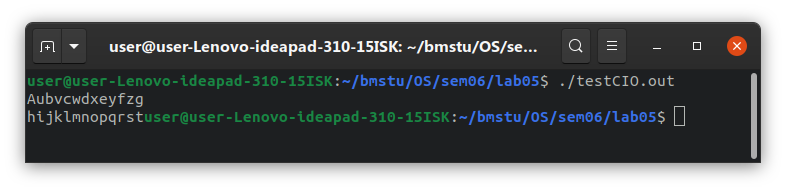
\includegraphics[width=\linewidth]{inc/img/testCIO-runtime}
	\caption{Демонстрация работы программы \code{testCIO.c}}
	\label{img:testCIO-runtime}
\end{figure}

\begin{figure}[H]
	\centering
	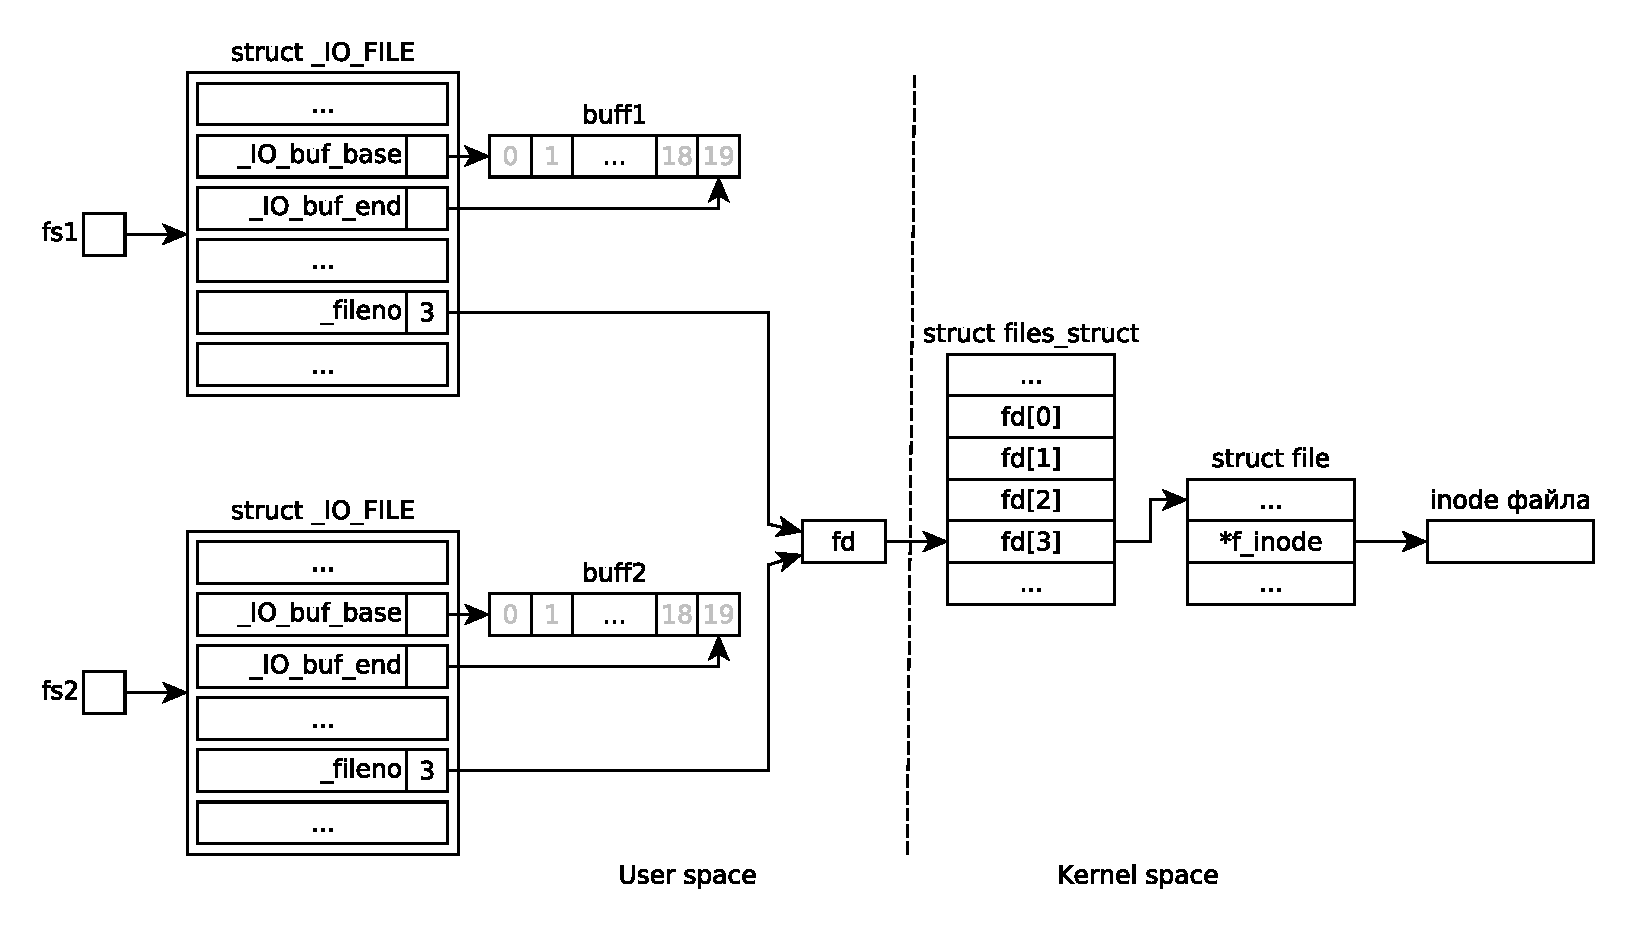
\includegraphics[scale=0.65]{inc/img/testCIO}
	\caption{Связь дескрипторов в \code{testCIO.c}}
	\label{img:testCIO}
\end{figure}

Системный вызов \code{open()} создаёт новый файловый дескриптор для открытого только на чтение (\code{O\_RDONLY}) файла \code{alphabet.txt}, запись в системной таблице открытых файлов.
Эта запись регистрирует смещение в файле и флаги состояния файла.
Новый файловый дескриптор является наименьшим дескриптором, который ещё не открыт процессом (\code{3}).
Функция \code{fdopen()} связывает потоки \code{fs1} и \code{fs2} с дескриптором \code{fd}.
Функция \code{setvbuf()} устанавливает блочную буферизации (\code{\_IOFBF}) размером 20 байт для каждого из потоков \code{fs1} и \code{fs2}.

Размер файла \code{alphabet.txt} составляет 27 байтов (26 букв английского алфавита и символ новой строки), в буфер потока \code{fs1} поместятся первые 20 байтов (\code{"Abcdefghijklmopqrst"}), в буфер потока \code{fs2} — оставшиеся 7 байтов (\code{"uvwxyz{\textbackslash}n"}).

В цикле чередуется вывод из потоков \code{fs1} и \code{fs2}.
Поскольку в буфере второго потока меньше символов, после последнего символа \code{'{\textbackslash}n'} выведутся оставшиеся в буфере первого потока символы.
Результат — строка \code{"Aubvcwdxeyfzg{\textbackslash}nhijklmnopqrst"}.

\section*{Программа 2}

\lstinputlisting[caption={testKernelIO.c}\label{lst:testKernelIO}, language=C]{../testKernelIO.c}

\begin{figure}[H]
	\centering
	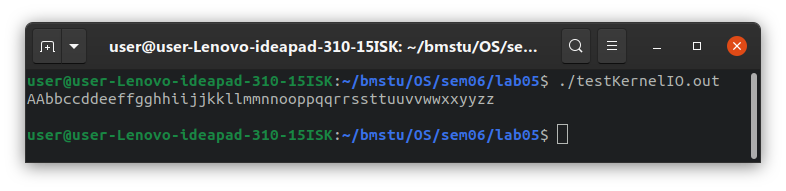
\includegraphics[width=\linewidth]{inc/img/testKernelIO-runtime}
	\caption{Демонстрация работы программы \code{testKernelIO.c}}
	\label{img:testKernelIO-runtime}
\end{figure}

\begin{figure}[H]
	\centering
	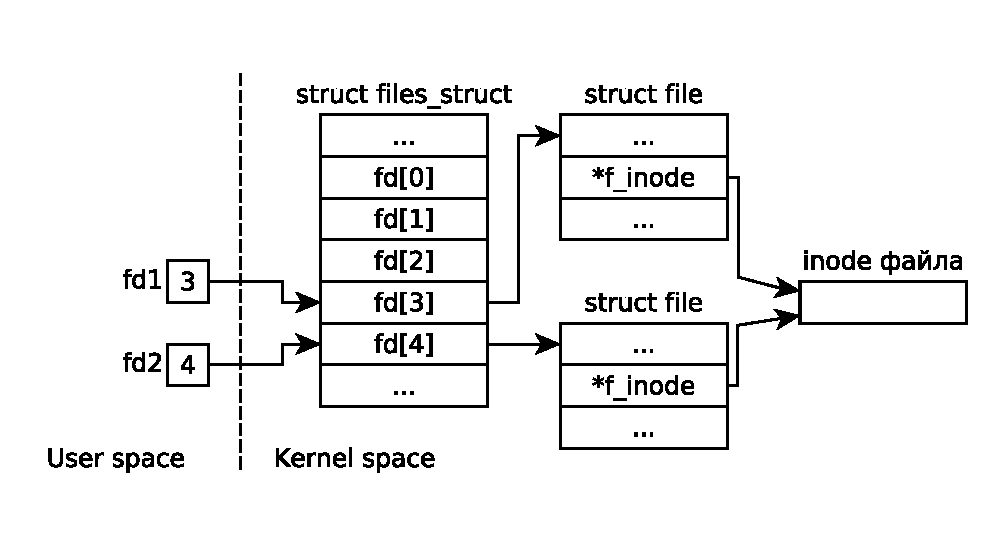
\includegraphics[scale=0.65]{inc/img/testKernelIO}
	\caption{Связь дескрипторов в \code{testKernelIO.c}}
	\label{img:testKernelIO}
\end{figure}

Файл \code{alphabet.txt} открывается системным вызовом \code{open()} только на чтение (\code{O\_RDONLY}) дважды, в системной таблице открытых файлов создаются две новых записи, дескрипторы помещаются в переменные \code{fd1} и \code{fd2} (хоть и описывают один файл, являются различными).
Смещения в файловых дескрипторах независимы, поэтому в цикле на экран выводится каждый символ из файла дважды.
Результат — строка \code{"AAbbccddeeffgghhiijjkkllmmnnooppqqrrssttuuvvwwxxyyzz{\textbackslash}n{\textbackslash}n"}.

\section*{Программа 3}

\lstinputlisting[caption={testCO.c}\label{lst:testCO}, language=C]{../testCO.c}

\begin{figure}[H]
	\centering
	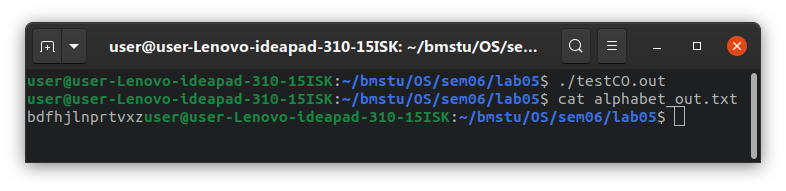
\includegraphics[width=\linewidth]{inc/img/testCO-runtime}
	\caption{Демонстрация работы программы \code{testCO.c}}
	\label{img:testCO-runtime}
\end{figure}

\begin{figure}[H]
	\centering
	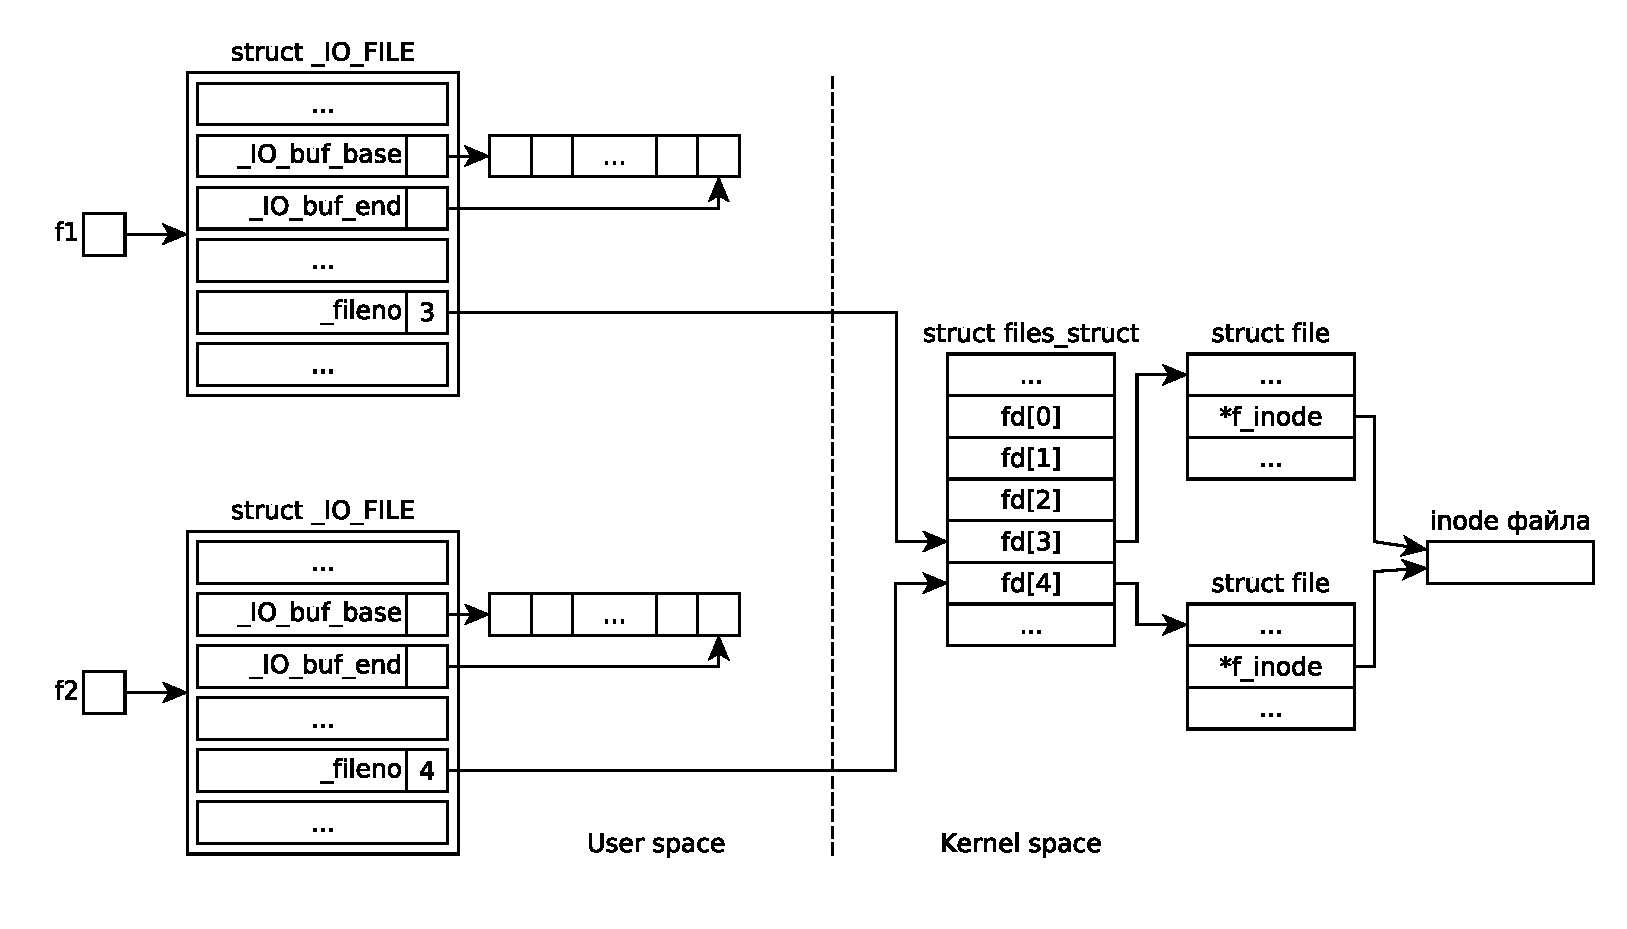
\includegraphics[scale=0.65]{inc/img/testCO}
	\caption{Связь дескрипторов в \code{testCO.c}}
	\label{img:testCO}
\end{figure}

Файл \code{alphabet\_out.txt} открывается функцией \code{fopen()} на запись дважды, в два различных потока \code{fs1} и \code{fs2}.

В цикле символы, имеющие нечётный код в таблице \code{ASCII}, записываются в буфер потока \code{fs1}, чётные — в буфер потока \code{fs2}.
После закрытия потока \code{fs1}, его буфер записывается в файл.
Смещения в потоках независимы, поэтому после закрытия потока \code{fs2}, его буфер записывается в файл опять с начала.
Результат — строка \code{"bdfhjlnprtvxz"}.

\section*{Cтруктура FILE}

\lstinputlisting[caption={FILE.h}\label{lst:FILE}, language=C]{../FILE.h}

\section*{Заключение}

Открытые файлы, для которых используется ввод/вывод потоков, могут буферизоваться.
Открытие одного и того же файла каждый раз создаёт новый файловый дескриптор и новую запись в системной таблице открытых файлов.
Эта запись регистрирует смещение в файле и флаги состояния файла.
Поэтому у различных дескрипторов открытого файла смещения не зависят друг от друга.

Чтобы избежать потери данных или получения неверного результата при буферизованном выводе в файл, необходимо учитывать то, что файл может быть открыт несколько раз, а также помнить о своевременном выполнении \code{fclose()} и \code{fflush()}.

\end{document}
